\section{Systems Modelling}

As the name suggests, systems modelling is the study of the conceptualisation and generation of models that can support the design and development of systems. This is a very large field with many different approaches that one can take to model a system. In this section, we will discuss three types that are commonly used within Engineering Design.

Function-flow\marginnote{Function-Flow} models attempt to describe the key dependencies and actions that occur within a systems architecture and there exist many methods of representing functions and flows.

The \ac{IDEF} is one such family of languages that is used to model manufacturing, information systems, business process and software engineering functions and was originally developed by the United States \ac{DoD}. 

IDEFO is the language used to create functional models where blocks represent decisions, actions and activities within a system (\cref{fig-idef0}). These blocks are then linked by their inputs, outputs and dependencies/influencers, and provides an overview of the flows within a system that one can analyse and interrogate further.

%https://upload.wikimedia.org/wikipedia/commons/thumb/3/31/IDEF_Diagram_Example.jpg/560px-IDEF_Diagram_Example.jpg
\begin{figure}[h!]
\centering
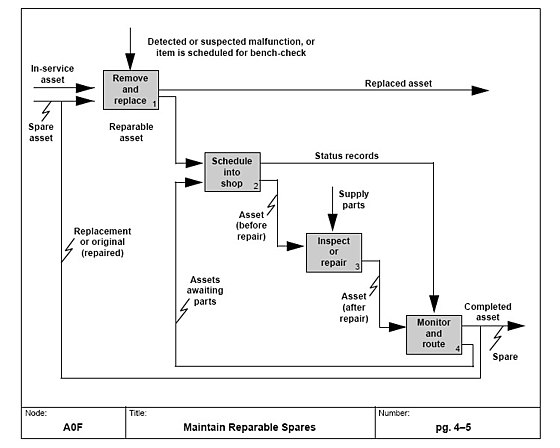
\includegraphics[width=0.9\textwidth]{figs/idef0.jpg}
\caption{An example of IDEF0}
\label{fig-idef0}
\end{figure}


%Icam Definition for Function Modelling (IDEF0) is a function modelling methodology often used in so
%\marginnote{Function-Flow}

Simulink\marginnote{Simulink} is a modelling language that features as part of MatLab (\cref{fig-simulink}). It uses block elements to represent physical systems and uses advanced solver technologies to show how a system will behave when perturbed.

\begin{figure}[h!]
\centering
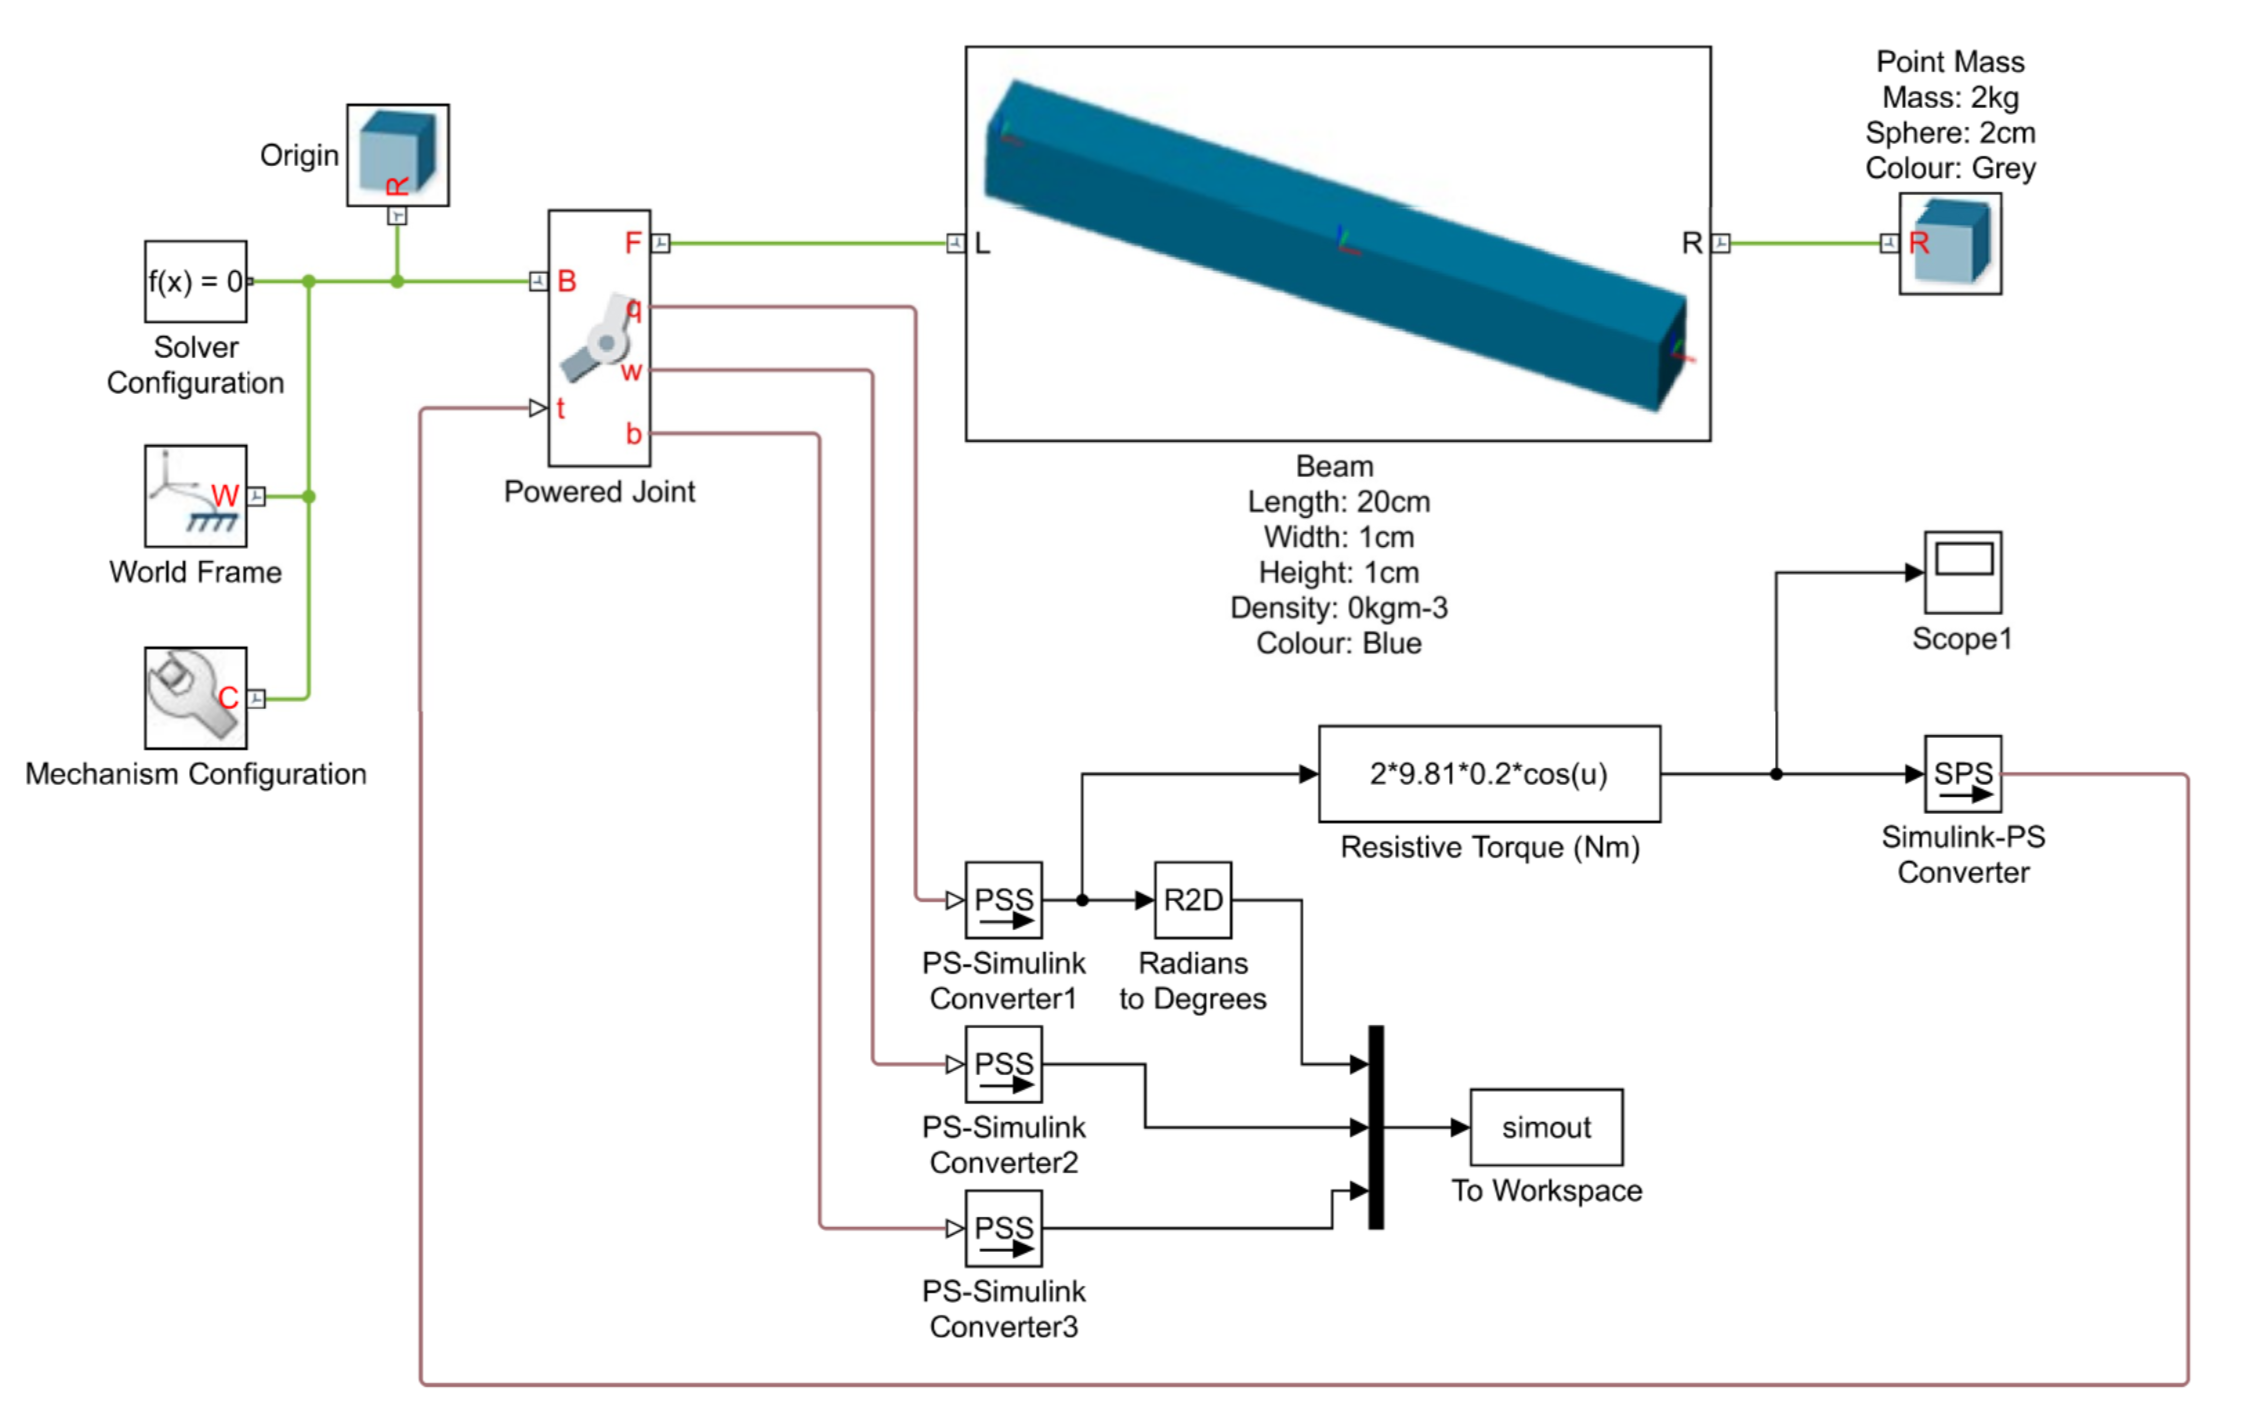
\includegraphics[width=0.95\textwidth]{figs/simulink.png}
\caption{Pendulum model in simulink}
\label{fig-simulink}
\end{figure}

In this exercise, we will be using Simulink to model our multi-bar mechanism that is being powered by its motor and gearbox. The key advantage of using the modelling software during the design of a product is that we can explore the optimum gear ratio and damping required for the mechanism to operate in a smooth and safe manner.

\ac{DSM}\marginnote{Design Structure Matrices} seek to understand the connected nature of engineering systems through a $N \times N$ matrix of interactions between system elements~\cite{eppinger2012}. The system elements can consist of individual components, assemblies of components, systems of components, engineers, teams of engineers, processes, and/or organisational structure to name a few. \ac{DSM}s enable engineers to analyse and visualize product, process, organisational, and multi-domain architectures of engineering products and projects.


The level of interactivity between elements being manually scored using either a range or binary set of values and are often generated from surveys and/or interviews with engineers across the company to determine the level of dependency between system elements\cite[-8em]{sosa2003}\cite[-2em]{gorbea2008}. 
From this, partitioning of the elements and matrix visualisation techniques are applied to enable insights to be drawn on the product/ organisational architecture. 
\citet{sosa2003} \ac{DSM} of a commercial jet engine (\cref{fig-sosa}) demonstrates the ability of \ac{DSM}s to identify key structures and insights, which were then used to support the design and development processes within the company.

\begin{figure}[h!]
\centering
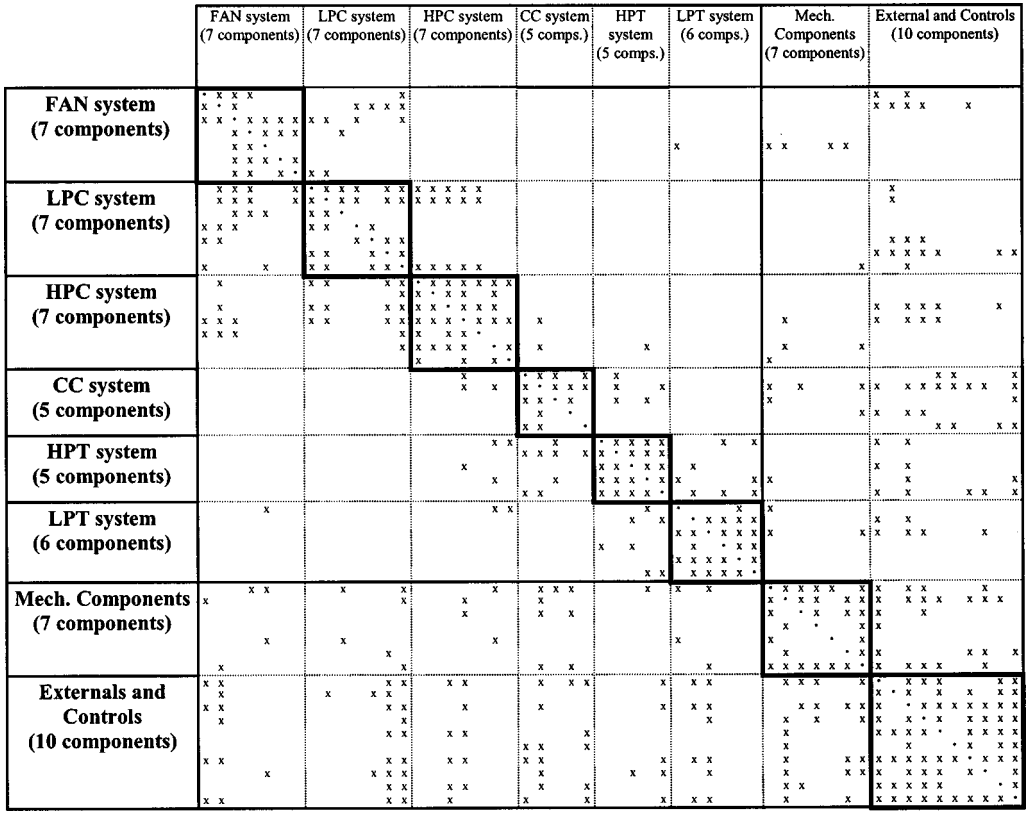
\includegraphics[width=0.9\textwidth]{figs/sosa-dsm.png}
\caption{The DSM of a Jet Engine}
\label{fig-sosa}
\end{figure}

In addition, analysis of these matrices can support the development of future design processes and build plans, and how changes to a component propagates changes to all the other components within a system\cite[-8em]{jarratt2011}.

Researchers\marginnote{research at bath} at Bath are leading the way in the development of a more automated and objective means of generating and assessing \ac{DSM}s\cite[-3em]{design2014}\cite{gopsill2016}. This is being achieved through the monitoring of meta-data changes to engineering files such as \acf{CAD}, \acf{CFD} and \acf{FEA}. 
Through monitoring the co-occurrence of changes between files (i.e.\ file B changing after file A), one can construct a statistical model of the dependencies between system elements as shown in Figure~\ref{fig-dsms}.

\begin{figure*}[h!]
\centering
\begin{tabular}{c c}
\subfloat[Initial DSM]{
  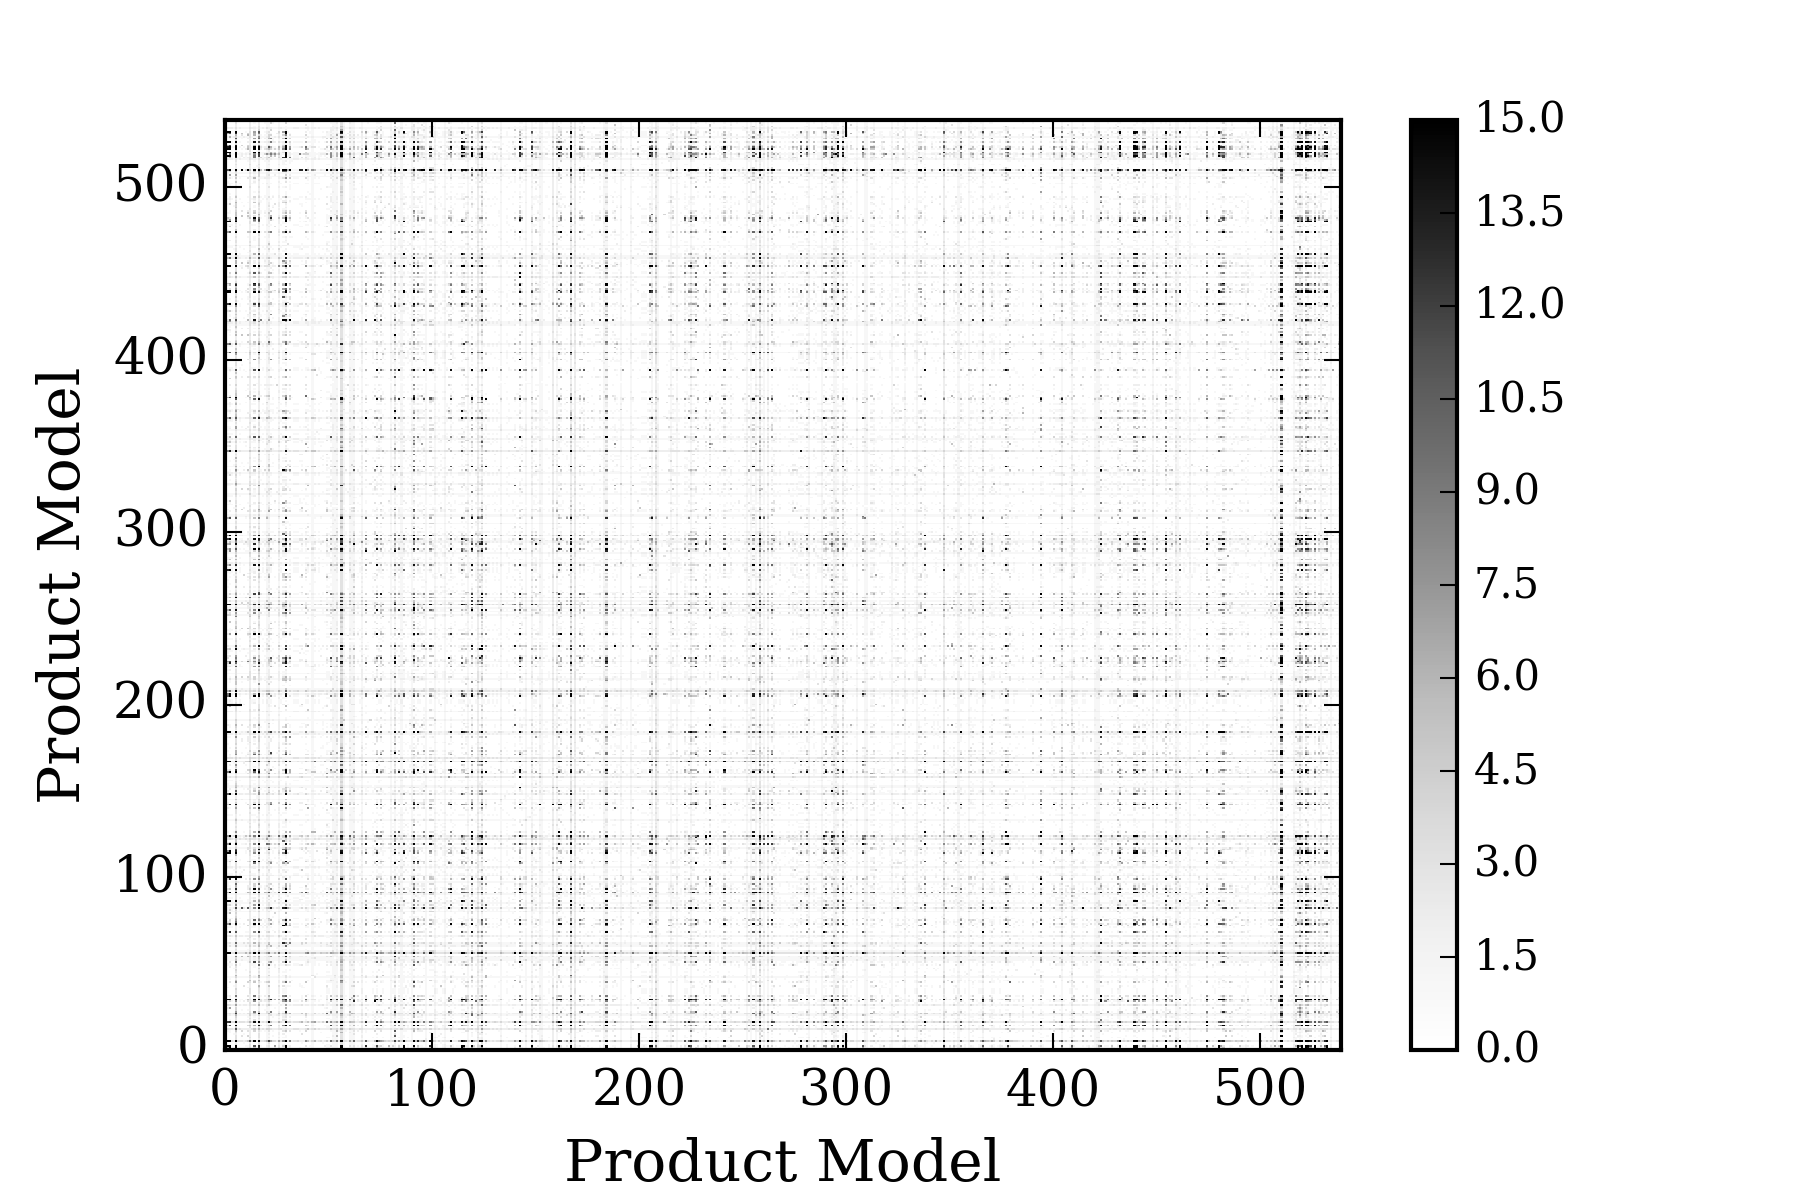
\includegraphics[width=0.45\textwidth]{figs/fs2013-14-initial-dsm.png}
} &
\subfloat[Partitioned DSM]{
  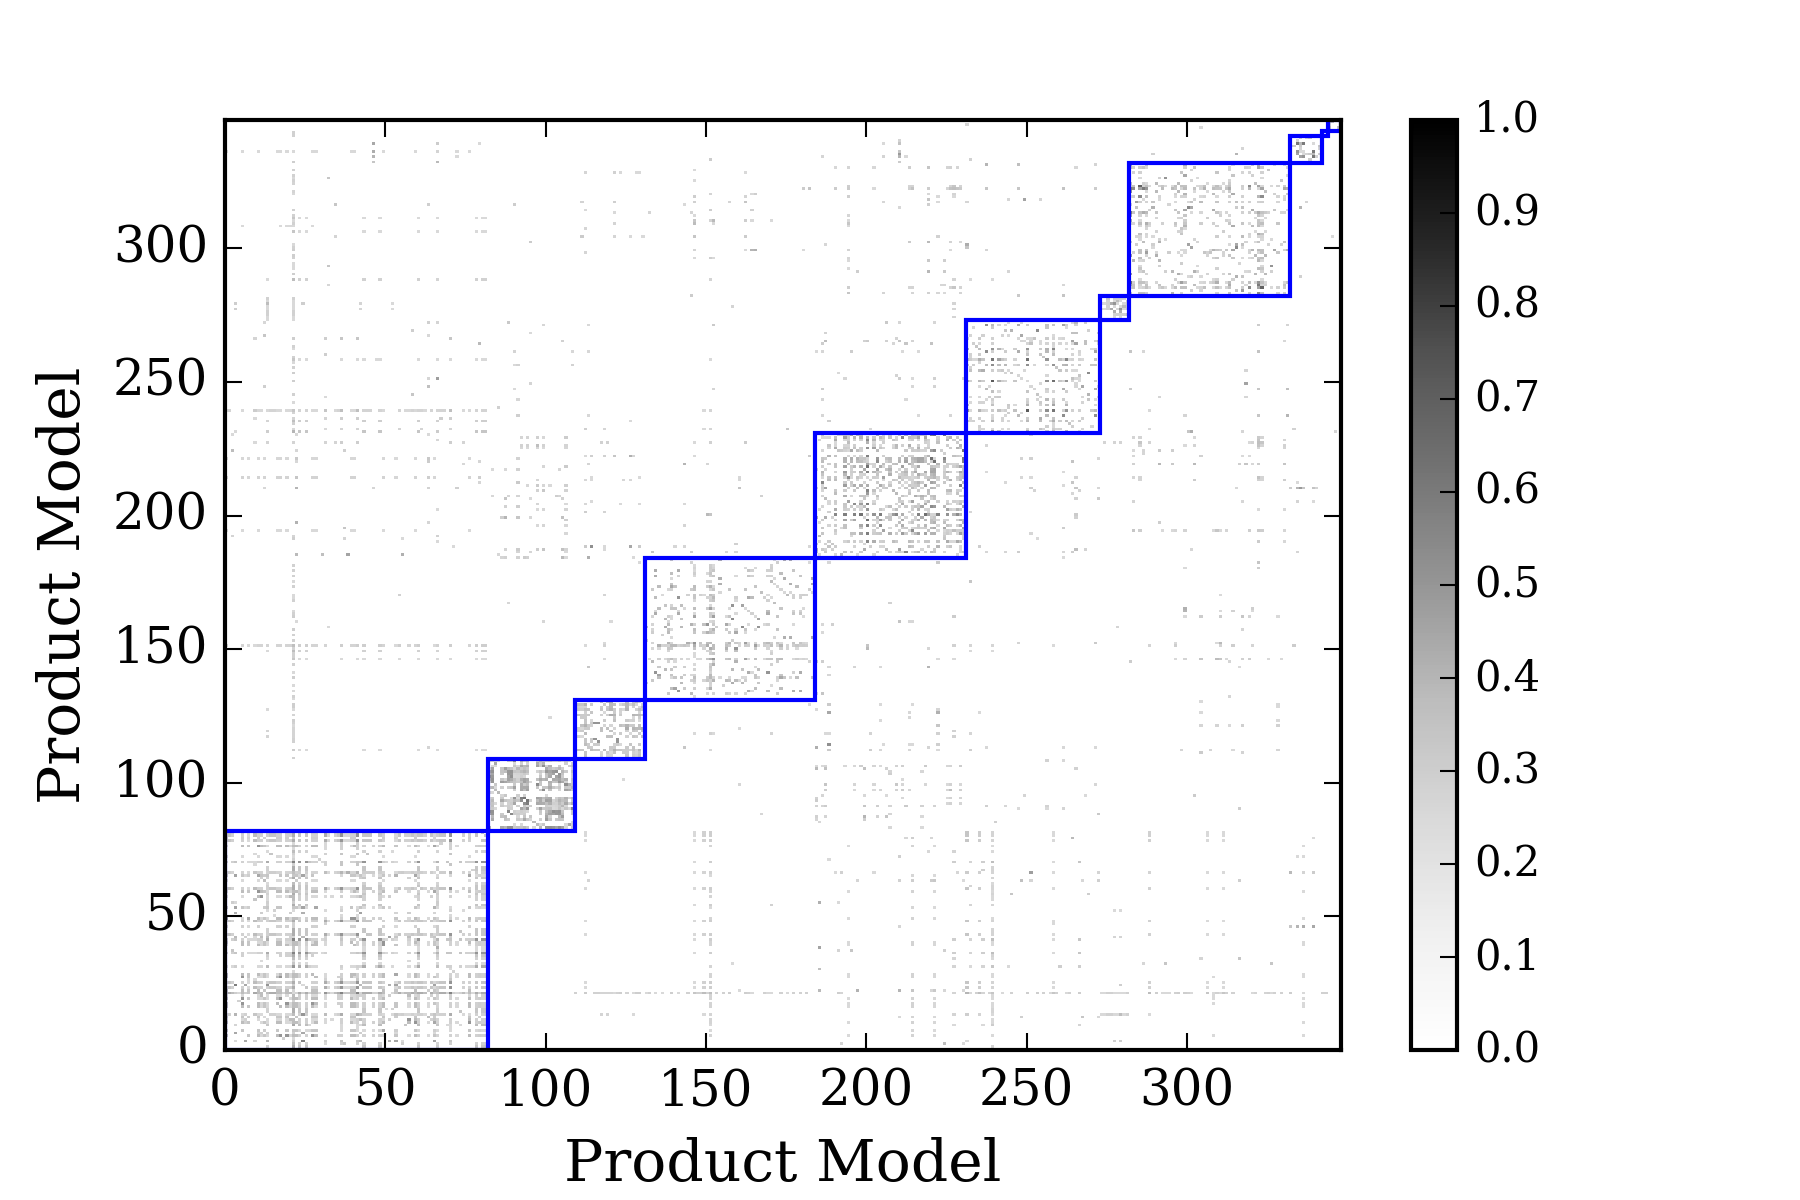
\includegraphics[width=0.45\textwidth]{figs/fs2013-14-clustered-dsm.png}
}\\
\end{tabular}
\vspace{1em}
\caption{Generating DSMs from the metadata changes of engineering files}
\label{fig-dsms}
\end{figure*}

The advantages of such a method is that it can maintain an up-to-date DSM as a engineering project evolves and the systematic nature of the process enables comparison of DSMs across projects.